
\section{Lecture 25: Static equilibrium, stability, rope walker}

We will begin by introducing the concept of static equilibrium. An object in static equilibrium is one that has no net force \emph{and} and no net torque (relative to any point we choose).\\
Such an object has zero linear acceleration and zero angular acceleration. In general, we will also assume they are at rest to begin with.\\
As an example, most objects on your table are likely in static equilibrium.

\begin{align}
\sum F &= 0\\
\sum \tau_Q &= 0 \text{ (any Q)}
\end{align}

For the net force to be zero, the net force must be zero along any axis by itself. Therefore, we can also use $\sum F_x = 0$, $\sum F_y = 0$ and $\sum F_z = 0$.

It might be easy to think that if the net force on a rigid object is zero, then it is in static equilibrium. That is far from true, though! If we have two forces of equal magnitude, acting in opposite directions, and they don't act along the same line, then they cause a net torque! The object will rotate, but will \emph{not} have any linear motion, since there is no net force.

\begin{center}
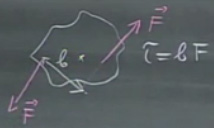
\includegraphics[scale=0.75]{\pIImages/lec25_couple}
\end{center}

(We can think of each force along causing a torque $(b/2) F \sin \theta$, where $\theta = \pi/2$ so $\sin(\theta) = 1$. They cause a torque in the same direction, so the total torque is $b F$.)

These two forces form a \emph{couple} (which I believe is a term used mostly in mechanics): together, they cause rotation, but \emph{not} translation.\\
An example of this are the forces exerted by your hand on a screw driver (or the forces exerted on the screw by the screw driver).

In this lecture, a ladder will be used for the calculations and examples regarding static equilibrium.

We put this ladder against a wall, at an angle $\alpha$ ($\alpha = 0$ meaning it is on the ground, while $\alpha = \ang{90}$ means it is standing straight up, parallel to the wall). Say there is no friction against the wall, but there is static friction $\mu$ at point Q, where the ladder touches the ground. We call the ladder's total mass $M$ and its length $\ell$.

\begin{center}
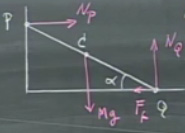
\includegraphics[scale=0.85]{\pIImages/lec25_ladder}
\end{center}

The center of mass of the ladder is in the middle.\\
Now... what forces act on this ladder?

First out, we have a gravitational force $M g$ acting on the center of mass.
 we have a normal force $N_Q$ where the ladder is in contact with the ground. Because the ladder wants to slide towards the right, there is a frictional force $F_f$ towards the left at point Q.\\
We said there is no friction at point P, so there can only be a normal force from the wall, towards the right; we call that $N_P$.

Let's now try to figure out when this static is in static equilibrium, i.e. at what angles $\alpha$ we can leave it, and have it be stable and remain at rest.\\
Our definition of static equilibrium was that the sum of all forces must be zero, and that the sum of all torques relative to any point must be zero. Let's first look at the forces.

First, in the $x$ direction. We have $N_P$ and $F_f$, so the two must be the same in magnitude.

\begin{equation}
N_P = F_f
\end{equation}

Next, the $y$ direction. Again, we have two forces, and find

\begin{equation}
N_Q = M g
\end{equation}

After this, we move on to torque. The torque relative to any point -- we can choose freely -- must be zero. If we choose point Q, neither $F_f$ nor $N_Q$ can contribute to the torque (since they act through point Q), and so we choose that point to simplify our lives.

First, we have the torque due to $N_P$. Torque is $\vec{r} \times \vec{F}$; the position vector from point Q has length $\ell$ (the entire ladder's length), and the angle between the two is $\alpha$. The cross product is then $\tau_{Q,N_P} = N_P \ell \sin \alpha$. The direction of this torque is into the blackboard, using the right-hand rule. We choose this as our positive direction, so this contributes a positive term to the net torque.

Next, there is a torque due to gravity pulling the ladder downwards. We model the gravity as acting purely at the center of mass, which is a length $\ell/2$ away from point Q. The angle between the two is not $\alpha$, but $\ang{90} - \alpha$. Therefore, the cross product becomes

\begin{equation}
\tau{Q,grav} = \frac{\ell}{2} M g \sin(\ang{90} - \alpha) = \frac{\ell}{2} M g \cos \alpha
\end{equation}

The direction is out of the blackboard, and so it contributes with a negative term. The two must be equal in magnitude, so

\begin{equation}
\sum \tau_Q = 0 \Rightarrow N_P \ell \sin \alpha = \frac{\ell}{2} M g \cos \alpha
\end{equation}

We can solve this for $N_P$:

\begin{equation}
N_P = \frac{M}{2} g \frac{\cos \alpha}{\sin \alpha} = \frac{M}{2} g \cot \alpha
\end{equation}

This must then be equal in magnitude to the frictional force, as we found earlier, or there will be a net force in the $x$ direction. This must always be smaller than the maximum possible static friction $\mu M g$, or the ladder will start to slide.

\begin{align}
\frac{M}{2} g \cot \alpha &\le \mu M g\\
\cot \alpha &\le 2 \mu\\
\alpha &\le \arctan \frac{1}{2 \mu}
\end{align}

The larger $\mu$ is, the smaller the angle can be without any sliding -- that is, the ladder can be closer to the ground, while still being held back by friction.\\
When $\mu$ is very small, it will slide at almost any angle, as we would expect. This is then demonstrated: smaller angles are less stable.

\subsection{Adding a mass along the ladder}

Let's now consider what happens when we actually use this ladder. Suppose we set it up just at the critical point, so that it is just about to slide. What happens if we stand near the bottom of the ladder, closer to point Q and far below the center of mass?\\
Will the ladder be more stable, less stable, or is there no change?

Let's consider what happens (rather quickly, as we will perform a full analysis soon). $N_Q$ will increase, which also increases the maximum possible frictional force $F_{fmax} = \mu N_Q$. This makes it seem likely that the ladder becomes more stable, as the maximum possible friction is now larger.\\
Since the actual friction $F_f = N_P$, has $N_P$ increased? I don't see why it would, so the system should become more stable.

What if the person keeps climbing, and moves past point C (the center of mass / center of the ladder), and keeps moving up towards point P? Is it now more stable, less stable, or does it not matter that the person is there?\\
Here (a bit unlike the previous case) I find it intuitively clear that this is \emph{not} a very safe thing to do. You add extra force downwards near the top of this about-to-fall ladder. This contributes to a torque that wants to rotate this ladder such that you fall down. It should also cause $N_P$ to increase, perhaps so that the required friction is now above the maximum possible. The system becomes less stable, as we will soon see.

We add a person of mass $m$ to the ladder, a distance $d$ away from point Q, measured diagonally along the ladder.

\begin{center}
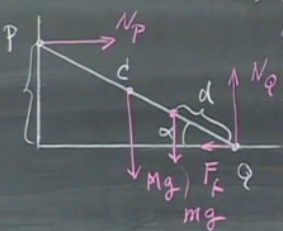
\includegraphics[scale=0.7]{\pIImages/lec25_ladder_person}
\end{center}

We then re-do the above calculations considering this extra mass.

For the $x$ direction, we still find $N_P = F_f$, as before.\\
In the $y$ direction, we have an extra downwards force, that $N_Q$ must balance out for the net force to be zero:

\begin{equation}
N_Q = (M + m) g
\end{equation}

This changes the maximum friction possible to

\begin{equation}
F_{fmax} = \mu N_Q = \mu (M + m) g
\end{equation}

which is clearly an increase from the previous case.\\
For the net torque, the first two terms are unchanged, but we add a third term due to the person of mass $m$ at distance $d$:

\begin{equation}
\sum \tau_Q = 0 \Rightarrow N_P \ell \sin \alpha = \frac{\ell}{2} M g \cos \alpha + m g d \cos \alpha
\end{equation}

The angle is calculated in the same way as last time. Again, we solve for $N_P$:

\begin{align}
N_P \ell \sin \alpha &= \frac{\ell}{2} M g \cos \alpha + m g d \cos \alpha\\
N_P \ell \sin \alpha &= g \cos \alpha \left(\frac{\ell}{2} M + m d\right)\\
N_P &= \frac{g \cos \alpha}{\ell \sin \alpha} \left(\frac{\ell}{2} M + m d\right)\\
N_P &= g \cot \alpha \left(\frac{M}{2} + \frac{m d}{\ell}\right)
\end{align}

And again, $N_P = F_f$ in magnitude, since they are the only two forces in the $x$ direction.

Since we have a new term $\displaystyle g \cot \alpha \frac{m d}{\ell}$, the frictional force has gone up. However, the maximum possible friction $F_{fmax} = \mu (M + m) g$ has also gone up!\\
In order to find which matters most, consider the case where the person is moving up the ladder gradually. To begin with, $d = 0$. We then gradually increase it. At $d = 0$, the frictional force has not changed at all, but the \emph{maximum possible} has! Therefore, the system is \emph{more stable} with this extra mass near the bottom. What happens as this mass is moving up along the ladder?

The maximum friction possible is independent of $d$, so that will always have the same, new value of $F_{fmax} = \mu (M + m) g$. However, as we climb, the actual frictional force $F_f = N_P$ (see above) does go up, due to new term we added.\\
When a certain point is reached, we are back to the just-about-to-slide situation again. If we climb higher yet, we are past that point, and the ladder will slide.

The condition we care about is that the frictional force is less than the maximum possible (when that is still the case, the ladder won't slide).

\begin{equation}
g \cot \alpha \left(\frac{M}{2} + \frac{m d}{\ell}\right) \le \mu (M + m) g
\end{equation}

However, we set the angle at the critical point we found earlier, where $\cot \alpha = 2 \mu$. We can substitute that in and solve for the largest $d$ possible for this inequality to hold:

\begin{align}
2 \mu \left(\frac{M}{2} + \frac{m d}{\ell}\right) &\le \mu (M + m)\\
M + \frac{2 m d}{\ell} &\le M + m\\
2 d &\le \ell\\
d &\le \frac{\ell}{2}
\end{align}

Quite an awesome result -- though perhaps one that could have been guessed, all things considered. Once we walk past (higher than) the center of mass, the situation is less stable that it was before. If we stand exactly \emph{at} the center of mass, we are at the just-about-to-slide stage. If we stand further down than the center of mass, the system is more stable than it was to begin with.

\section{Rope around a cylinder (capstan equation)}

We can often use friction to our advantage. One example of such a case is often used by sailors: by wrapping a rope around a cylinder, we can use friction forces as a ``substitute'' for string tension. We can have a very large force pulling on one end of the rope, which is countered in part by tension on the other side of the rope, but in larger part due to friction between the rope and the cylinder it is wrapped around.

\begin{center}
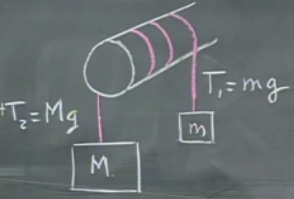
\includegraphics[scale=0.75]{\pIImages/lec25_capstan}
\end{center}

Here, we have two masses attached to either end of a rope. The middle part of the rope is wrapped several times around a cylinder.\\
If the system is at rest, $T_1 = M g$ and $T_2 = m g$. The mass $M$ is much greater than the mass $m$.

The reason the system can be at rest under these circumstances is that friction between the cylinder and the rope is trying to hold the rope in place. 

\begin{center}
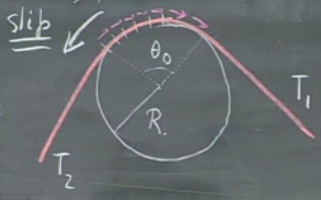
\includegraphics[scale=0.7]{\pIImages/lec25_capstan2}
\end{center}

If we consider the friction at the surface of each tiny length element of the rope, it is clear that the rope wants to slip towards the left (counterclockwise), and therefore, friction is attempting to oppose this motion. $T_2$ is pulling towards the right, but $T_1$ \emph{plus} the total frictional force is pulling towards the right. With enough friction, $T_1$ can be very small compared to $T_2$ and we can still have static equilibrium.

The result (the derivation is fairly complex and thus not shown) is that the ratio of the two tensions is given by

\begin{equation}
\frac{T_2}{T_1} = e^{\mu \theta_0}
\end{equation}

where $e^x$ is the exponential function, $\mu$ is the coefficient of static friction between the rope and the cylinder, and $\theta_0$ is the angle over which the rope is in contact with the cylinder. There is no particular limit on this angle: it could be wrapped 10 turns, which would make $\theta_0 = 20 \pi$.\\
This is known as the \emph{capstan equation}. My dictionary says that a capstan is ``a revolving cylinder with a vertical axis used for winding a rope or cable, powered by a motor or pushed around by levers''.

Notice that this result is independent of the cylinder's radius; only the angle matters.\\
The result is also exponential, so it grows extremely quickly. Adding an extra turn can make a tremendous difference in the tension ratio. For example, consider $\mu = 0.3$.

If we wrap it around exactly once, the ratio is $\displaystyle \frac{T_2}{T_1} = 6.59$ (already an impressive number). Two turns makes the ratio $43.38$, three turns $285.7$... eight turns $\num{3.54e6}$! So the first mass could be one ton, and in theory the tension from a second mass of less than one gram would be enough to counter it. Clearly, we wouldn't need to go to such extremes for this to be very useful. A mere 4 turns is enough for 1 kg to counter more than 1800 kg (or 1 N to counter more than 1800 N; since the ratio is all that matters, we can compare hanging masses in kg and tensions in newton just the same).

Let's go back to a less extreme example. If $\mu = 0.2$ and we wrap the rope 6 turns around, the ratio is about 1881, call it 2000. (If $\mu = 0.202$ instead, it goes above 2000, so it's certainly not far from it!)

With a 10 000 kg mass $M$ hanging on the left side, we could balance that force with a $\SI{10000}{kg}/2000$ = 5 kg mass on the right side! Alternatively, we could hold the rope in our hands and have no problem at all balancing this 10 ton mass on the other side.

What would happen if we let go just a little, and reduced our force from the approximately 50 newtons $(\SI{5}{kg}) g$ to just a tiny bit less? Since this ratio is for the no-slip condition, it will start to slip, and the huge mass will win, and move downwards. We can therefore control this large mass, and lower it down gently, with barely any force at all exerted by us.

What about raising the mass up? We now run in to a problem... a very, very big problem. We now want the rope to slip in the opposite direction, so that it comes towards us. This means that all those tiny friction elements between rope and cylinder switch direction, to as always oppose the relative motion between the two surfaces. To lift this object up, we must now overcome that friction \emph{and} the object's weight... so we must provide a force \emph{2000 times larger} than the object's weight in order to move it, which for a 10 ton mass is the same as hanging a 20 000 ton (20 million kg) mass on this side!\\
We should perhaps stick to lowering things down (and balancing things) using this mechanism.

This (balancing a heavy object) is then demonstrated, with a mass of approximately 30 kg hanging from a rope. After winding the rope a few times around a cylinder, the mass hangs there with almost no counterbalancing force at all. With 12 windings (perhaps even less, as 9, 10 or 11 was not tested) the weight of the remaining rather thin rope itself was enough to balance the 30 kilograms without having to even touch the rope.

\subsection{More on static equilibrium}

Consider an object of some shape (any shape), hanging on a pin somewhere (somewhere that is not through the center of mass, or the point of this will be lost).

\begin{center}
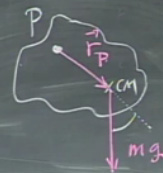
\includegraphics[scale=0.75]{\pIImages/lec25_com_position}
\end{center}

Gravity acts on the center of mass, which is not located at point P, so there will clearly be a torque. The object will start to rotate, and practically become a pendulum. Suppose we either wait until friction takes care of that, or we stop it manually. Clearly, at some point, it will reach a static equilibrium and stand completely still.

This can only happen when the center of mass is on a straight, vertical line with the point P from which it is suspended. In any other case, $\vec{r_P} \times \vec{F_{grav}} \neq 0$ and so there is a torque relative to point P, causing it to rotate.\\
More specifically, the only stable situation occurs when the center of mass is straight \emph{below} the point of suspension. Any time it is straight \emph{above}, any tiny disturbance will of course cause it to turn 180 degrees and then (once stopped) be in static equilibrium like that, instead.

We can then use this information to determine the center of mass very easily (at least in the case of a practically two-dimensional object). We hang it from one location, and draw a line from the pin (that we hang it from) and straight downwards.\\
We then move the pin to some other location, let it settle, and again draw a line straight downwards.

Since the center of mass must have been straight below the point in both two cases, there will be a unique point where the two lines intersect, where the center of mass is located!\\
Clearly, we can't find it from a single measurement: we only know that it will be straight below; it could be \emph{anywhere} straight below though (within reason -- it can't be below the lowest point of the object, of course)! With two measurements, we can narrow it down to a point on a 2D surface.

\section{Lecture 26: Elasticity and Young's Modulus}

We will now look at elasticity in materials. First, we will look at a similar situation with springs and Hooke's law.

Say we have a regular spring, with length $\ell$ and spring constant $k$. We extend it a length $\Delta \ell$ past its natural length, and according to Hooke's law, the spring force is $-k \Delta \ell$ -- a force which is trying to return the spring to its natural length. If we pull twice as hard, $\Delta \ell$ will double, and the spring force will also double.

Now, consider instead doubling the natural length of the spring. For the same pulling force, we now get twice the extension $\Delta \ell$. We can consider this as having two identical springs in series, instead of doubling the length of one, as the physics are the same. Each spring will experience the same pulling force, and so each spring individually will get longer by $\Delta \ell$. Therefore, the spring that is twice as long is extended twice as much.

If we instead have two (still identical) parallel springs, i.e. two springs are fastened at some wall, while a block or such is put on the other side and attached to each spring individually, they will have to share the load. Therefore, if we pull with a force $F$, each spring will respond with a force $-F/2$, so that the net force due to the two springs cancels out our pulling force.\\
Since they are still identical, with the same $k$, they must each be extended by only half as much as previously, so that the sum of the force due to both springs equals the pulling force.\\
If we had three springs in parallel, each would only have to provide a third of the force, and would only extend a third as much.

With these short thought experiments in mind, we have found these three relationships for these springs:

\begin{align}
\Delta \ell &\propto F\\
\Delta \ell &\propto \ell\\
\Delta \ell &\propto \frac{1}{\text{\# of springs in parallel}} \text{ (for identical springs)}
\end{align}

Let's now move on to the subject at hand. We replace the springs by rods (say metal rods, for example) with a cross-sectional area $A$ and length $\ell$. We apply a force at one end of the rod (while it is fastened at the other end, like the springs).

If we new consider this rod as a spring, pulling on this rod with a force $F$ will again extend it a distance $\Delta \ell$. As long as Hooke's law holds, i.e. that the restoring force is proportional to $\Delta \ell$, we can again say that $\Delta \ell \propto F$.

What if we put two rods together, so that the length doubles? (That is, we put them ``in series''.)\\
Again, we get the same result: each rod experience the force $F$, so each rod extends by $\Delta \ell$, and the extension doubles by doubling the length of the rod. $\Delta \ell \propto \ell$ holds for the rods, too.

Finally, what if we have two next to each other, in parallel? We pull downwards with a force $F$, that is shared by the two rods. Each rod only needs to counter half of our pull, and so they extend by $\Delta \ell/2$, just like the springs did. With twice the cross-sectional area $A$ of the rods, we get half $\Delta \ell$. Therefore, $\Delta \ell$ is inversely proportional to the cross-sectional area of the rods.

All in all, for the rods, we find

\begin{align}
\Delta \ell &\propto F\\
\Delta \ell &\propto \ell\\
\Delta \ell &\propto \frac{1}{A}
\end{align}

We can write this as a single proportionality:

\begin{equation}
\Delta \ell \propto \frac{F \ell}{A}
\end{equation}

Reordered,

\begin{equation}
\frac{F}{A} \propto \frac{\Delta \ell}{\ell}
\end{equation}

The proportionality constant $Y$ (or $E$) is called Young's modulus. The equation becomes

\begin{equation}
\frac{F}{A} = Y \frac{\Delta \ell}{\ell}
\end{equation}

Because the fraction on the right has no dimension, while the left-hand side has dimension force per unit area, which is pressure, $Y$ also has units of pressure (newtons per square meter).

In this equation, $\displaystyle \frac{F}{A}$ is called the \emph{stress} while $\displaystyle \frac{\Delta \ell}{\ell}$ is known as \emph{strain}.

If we compare two rods with different value for Young's modulus, the one with the smaller value is easier to stretch out: it gives a larger strain for a given stress. If the Young's modulus is very high, the rod is very stiff.

As an example, if we hang a mass of 500 kg of a cylindrical steel rod of radius 0.5 cm and length 1 meter, how much will it stretch? We can start by solving the equation for $\Delta \ell$:

\begin{equation}
\frac{F \ell}{A Y} = \Delta \ell
\end{equation}

$F = (\SI{500}{kg})(\SI{10}{m/s^2}) = 5000$ N. $A = \pi R^2 = \SI{7.85e-05}{m^2}$. $Y$ for steel is given as $\SI{20e10}{N/m^2}$. We find $\Delta \ell = 0.32$ mm.\\
If we instead use nylon with $Y = \SI{0.36e10}{N/m^2}$, it would stretch 18 mm.

The stress in this case is about $\SI{6.4e7}{N/m^2}$ (for either material -- it does not depend on $Y$, only on the force and the cross-sectional area).

If we keep adding more mass, there is clearly a point where the rod will simply break. That breaking point is at the \emph{ultimate tensile strength}, which is given as a pressure. In other words, when $\displaystyle \frac{F}{A}$ becomes too large, the rod breaks.\\
The ultimate tensile strength of both steel and nylon are such that neither would break given the load we calculated above; even the nylon could tolerate a few times this force. If the bar was made out of aluminium however, which has an ultimate tensile strength of about $\SI{7.8e7}{N/m^2}$, we would be rather close to the breaking point.

Before the material breaks, our equation will stop working, as the strain will no longer be proportional to the stress. Hooke's law no longer holds. If we overload the material like that, it will not return to its original length again, but will be permanently deformed. This also has an analogue with springs: pull too much on a spring, and the restoring force becomes nonlinear, and the spring will eventually be permanently deformed.

Let's have a look of what a stress vs strain plot may look like.

\begin{center}
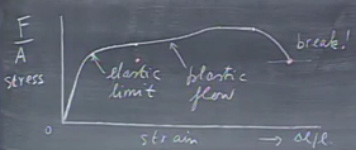
\includegraphics[scale=0.75]{\pIImages/lec26_stress_vs_strain}
\end{center}

The first part of the curve is linear: this is where Hooke's law applies. The next part of the curve is nonlinear, and goes to a point known as the \emph{elastic limit}. Even though it is not linear, as long as we do not pass the elastic limit, the material will return to its original length after we return the force.

Once we pass the elastic limit, however, the material will be permanently deformed.\\
Past this limit, increasing the stress by small amounts will cause very large amounts of strain: That is, the material will be much easier to stretch. If we then remove the force, the material would not return back to where it was. That also implies that if we create a graph like this one by gradually increasing the force and plotting $\displaystyle \frac{\Delta \ell}{\ell}$, if we gradually remove the force, the strain will not follow the curve back to zero, but will instead return to somewhere to the right of the origin.\\
The work we have done in pulling will go in part to deforming the rod, which takes energy, and in part to heat: the rod will heat up, sometimes quite substantially.

Past the elastic limit, but before the breaking point, there is a completely horizontal part of the curve. This implies that with no change at all in the stress ($y$ axis), the strain will increase anyway, and the rod will stretch without any extra force being applied. We call this \emph{plastic flow}. In this region, the material acts almost like a liquid, flowing towards the force.

Prior to breaking, the stress is lower than it was in the plastic flow region. The reason is that the material can start to pinch, so that it gets thinner at a point. That will cause the cross-sectional area to decrease, and so $\displaystyle \frac{F}{A'}$, where $A'$ is the new cross-sectional area, will be larger than $\displaystyle \frac{F}{A}$ for other points.

There are machines designed to test materials, and create plots like this one. They then increase the value of $F$ very gradually, and measure the strain. In the linear region, and the nonlinear region around the elastic limit, this is straightforward.\\
Once they start reaching the plastic flow area, however, they decrease the force. If $\Delta \ell$ increases anyway, they decrease it further. It then becomes possible to trace out the entire curve, until the breaking point.

Brittle materials generally have a curve with many of the same characteristics, but they are practically squashed together right-to-left, so that all these regions occur for smaller values of the strain.

Next we have a very long demonstration with a set-up and measuring of these values of strain vs stress, and plotting them on the blackboard. As usual, I don't really take any notes during demonstrations.

As one of many results of the demonstration, we find that in the linear region, the 36 cm copper rod has only expanded with about 0.13\%. Any further expansion was not linear, and eventually entered the plastic flow region, where adding 1 kg more (for a total of 5 kg) hanging from the copper string would \emph{double} $\Delta \ell$ -- not very linear at all!

A typical breaking point for metals would be at 5\% to 10\% extension over the original length, or so.

\subsection{Elasticity and simple harmonic oscillations}

In the linear portion, just as with springs, there is a restoring force that is linearly proportional.to the extension distance. Assuming this also holds for compression (which appears to have been silently assumed in the lecture), this forms a simple harmonic oscillator. We can solve the equation regarding the Young's modulus for $F$:

\begin{align}
F = \frac{A Y}{\ell} \Delta \ell
\end{align}

Here, we can think of $\displaystyle \frac{A Y}{\ell}$ as the spring constant $k$ (the units are indeed N/m), while as we saw earlier in the lecture $\Delta \ell$ is really just a different way of notating the displacement $x$. Stick a minus sign in there to take care of the direction (it's a restoring force), and we have an equation that is the same as that of a spring oscillator with $\displaystyle k = \frac{A Y}{\ell}$, which gives us

\begin{align}
\omega &= \sqrt{\frac{k}{m}} = \sqrt{\frac{A Y}{\ell m}}\\
T &= \frac{2 \pi}{\omega} = 2 \pi \sqrt{\frac{\ell m}{A Y}}\\
f &= \frac{\omega}{2 \pi} = \frac{1}{2\pi} \sqrt{\frac{A Y}{\ell m}}
\end{align}

For $Y = \SI{11e10}{N/m^2}$, $m = 3$ kg, $A = \SI{2e-7}{m^2}$ and $\ell = 0.36$ m, we find a frequency of about 23 Hz.
